\documentclass{article}
\usepackage{graphicx}
\usepackage{amsmath}
\usepackage{amssymb}

\title{Simulation Write Up}

\begin{document}
\maketitle

\section{Data Generating Process}

The causal DAG for the data generating process is given as 
\begin{center}
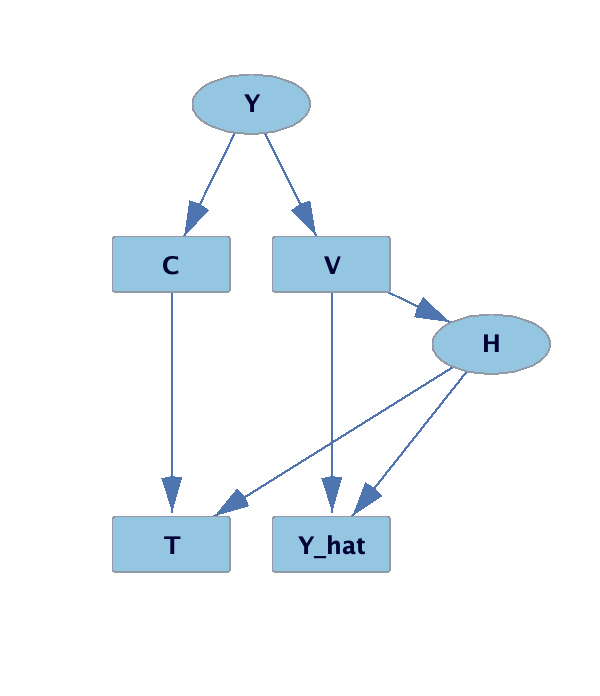
\includegraphics[scale = 0.5]{true_dgp.png}
\end{center}

And since $Y$ and $H$ are latent, when we run FCI with this graph we obtain the following output, and this is after applying knowledge that Y$\_$hat is in a later tier than the rest.

\begin{center}
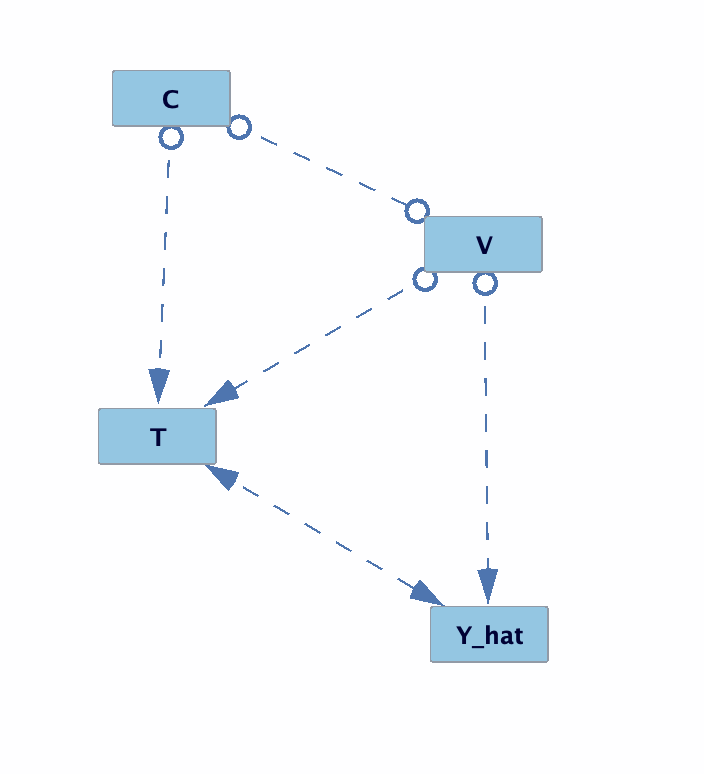
\includegraphics[scale=0.4]{FCI_output_true_dgp.png}
\end{center}

\section{Simulation Parameters}

The following parameters are used to simulate the shapes in the images, along with each image being given random noise in the background as well.
\begin{align*}
Y &\sim Bernoulli(0.5)\\
C & \sim expit(-1 + 2.5*Y)\\
T &\sim expit(1 + C+ H)\\
V &\sim expit(-1.5 + 3.18*Y)\\
\end{align*}

We want our simulation to obey the following properties:
\begin{itemize}
\item  We want $P(Y = 1 \mid V = 1)$ to be high, and we want $P(Y = 1 \mid V = 0)$ to be low. 
\item Inversely, we want, $P(Y = 1 \mid H = 1)$ to be low, and $P(Y = 1 \mid H = 0)$ to be high. 
\end{itemize}

First to demonstrate the current simulation parameters for $V$ do give us the desired property. Based on the simulation parameters: $p( V = 0 \mid Y = 1) = 0.1571$ and $p(V = 0 \mid Y = 0) = 0.8175$
\begin{align*}
p(Y = 1 \mid V = 0) &= \frac{p(V = 0 \mid Y = 1) p(Y = 1)}{p(V = 0 \mid Y = 1) p(Y = 1) + p(V = 0 \mid Y = 0) p(Y = 0)}\\
&= \frac{p(V = 0 \mid Y = 1)}{p(V = 0 \mid Y = 1) + p(V = 0 \mid Y = 0) }\\
&= \frac{0.1571}{0.1571 + 0.8175} = \frac{0.1571}{0.9746} = 0.1611\\
p(Y = 1 \mid V = 0) &= 0.1611
\end{align*}

Doing a similar computation for $p(Y = 1 \mid V = 1)$, and using $p(V = 1 \mid Y = 1) = 0.8429$ and $p(V = 1 \mid Y = 0) = 0.1824$
\begin{align*}
p(Y = 1 \mid V = 1) &= \frac{p(V = 1 \mid Y = 1) p(Y = 1)}{p(V = 1 \mid Y = 1) p(Y = 1) + p(V = 1 \mid Y = 0) p(Y = 0)}\\
&= \frac{p(V = 1 \mid Y = 1)}{p(V = 1 \mid Y = 1) + p(V = 1 \mid Y = 0)}\\
&= \frac{0.8429}{0.8429 + 0.1824} = \frac{0.8429}{1.0253} = 0.8221\\
p(Y = 1 \mid V = 1) &= 0.8221
\end{align*}

So $Y$ is positively correlated with the presence of V-bars. Now we want the opposite for H-bars, and we must choose simulation parameters for H accordingly. First, note
\begin{align*}
p(Y = 1 \mid H = 0) &= \sum_{V} p(Y = 1 \mid V, H = 0)p(V \mid H = 0)\\
&= p(Y = 1 \mid V = 0, H = 0)p(V = 0 \mid H = 0) \\ &
+ p(Y = 1 \mid V = 1, H = 0)p(V = 1 \mid H = 0)
\intertext{Since $Y \perp H \mid V$, the above becomes}
&= p(Y = 1 \mid V = 0)p(V = 0 \mid H = 0) + p(Y = 1 \mid V = 1)p(V = 1 \mid H = 0)\\
&= 0.1611*p(V = 0 \mid H = 0) + 0.8221*p(V = 1 \mid H = 0)\\
p(Y = 1 \mid H = 0) &= 0.1611*(1 - p(V = 1 \mid H = 0)) + 0.8221*p(V = 1 \mid H = 0)\\
\end{align*}

Since we want $p(Y = 1 \mid H = 0)$ to be high, we want $p(V = 1 \mid H = 0)$ to be high as well. Performing a similar calculation for $p(Y = 1 \mid H = 1)$, we have
\begin{align*}
p(Y = 1 \mid H = 1) &= \sum_{V} p(Y = 1 \mid V, H = 1)p(V \mid H = 1)\\
&= p(Y = 1 \mid V = 0, H = 1)p(V = 0 \mid H = 1) \\ &
+ p(Y = 1 \mid V = 1, H = 1)p(V = 1 \mid H = 1)\\
&= p(Y = 1 \mid V = 0)p(V = 0 \mid H = 1) + p(Y = 1 \mid V = 1)p(V = 1 \mid H = 1)\\
&= 0.1611* (1 - p(V = 1 \mid H = 1)) + 0.8221*p(V = 1 \mid H = 1)
\end{align*}

Since we want $p(Y = 1 \mid H = 1)$ to be low, we want $p(V = 1 \mid H = 1)$ to be low. Applying Bayes Theorem to obtain $p(V = 1 \mid H = 1)$ and $p(V = 1 \mid H = 0)$ we can write
\begin{align*}
p(V = 1 \mid H = 0) &= \frac{p(H = 0 \mid V = 1)p(V = 1)}{p(H = 0 \mid V = 0)p(V = 0) + p(H = 0 \mid V = 1)p(V = 1)}\\
p(V = 1 \mid H = 1) &= \frac{p(H = 1 \mid V = 1)p(V = 1)}{p(H = 1 \mid V = 0)p(V = 0) + p(H = 1 \mid V = 1)p(V = 1)}
\end{align*}

Consequently, need to calculate $p(V)$, done below:
\begin{align*}
p(V = 0) &= p(V = 0 \mid Y = 0)p(Y = 0) + p(V = 0 \mid Y = 1)p(Y = 1)\\
&= 0.8175*0.5 + 0.1571*0.5 = 0.5*0.9746 = 0.4873\\
\end{align*}

And similarly,
\begin{align*}
p(V = 1) &= p(V = 1 \mid Y = 0)p(Y = 0) + p(V = 1 \mid Y = 1)p(Y = 1)\\
&= 0.1824*0.5 + 0.8429*0.5 = 0.5126
\end{align*}

Plugging into the above formulas
\begin{align*}
p(V = 1 \mid H = 0) &= \frac{p(H = 0 \mid V = 1)*0.5126}{p(H = 0 \mid V = 0)*0.4873 + p(H = 0 \mid V = 1)*0.5126}\\
p(V = 1 \mid H = 1) &= \frac{p(H = 1 \mid V = 1)*0.5126}{p(H = 1 \mid V = 0)*0.4873 + p(H = 1 \mid V = 1)*0.5126}
\end{align*}

And so, we want $p(H = 0 \mid V = 1)$ high, as well as $p(H = 1 \mid V = 0)$ to be high as well. This translates into $p(H = 1 \mid V = 1)$ being small, and $p(H = 1 \mid V = 0)$ being big - which requires a strong negative correlation. For this reason, the following parameters are chosen for generating H
\begin{equation*}
H \sim expit(2.5 - 4.7*V)
\end{equation*}

\section{Updated Round of Simulations In Light Of Issues}
The updated causal DAG for the data generating process is given as 
\begin{center}
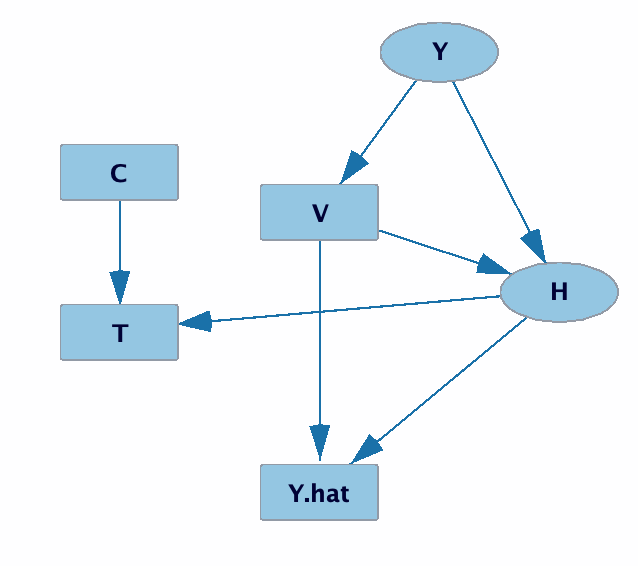
\includegraphics[scale = 0.5]{updated_DGP.png}
\end{center}

When $\hat{Y}$ is generated using a logistic regression, it can be written as $\mathbb{I}(expit(\beta_0 + \beta_1*V + \beta_2*H) \geq 0.5)$. Now to avoid collinearity with $V$, we want to set up $\beta$ such that $V$ alone can't make the expit value positive. Tis results in the desired probability distribution:
\begin{align*}
\mathbb{P}(\hat{Y} = 1\mid H = 0, V = 0) &= 0\\
\mathbb{P}(\hat{Y} = 1\mid H = 1, V = 0) &= 0\\
\mathbb{P}(\hat{Y} = 1\mid H = 0, V = 1) &= 0\\
\mathbb{P}(\hat{Y} = 1\mid H = 1, V = 1) &= 1\\
\end{align*}

To avoid collinearity between $\hat{Y}$ and $V$, we must avoid the situation of $\mathbb{P}(\hat{Y} = 1\mid V = 1)$ and $\mathbb{P}(\hat{Y} = 1\mid V = 0)$ being degenerate. So, to compute $\mathbb{P}(\hat{Y} = 1 \mid V) = \sum_{H}\mathbb{P}(\hat{Y} = 1 \mid V, H)\mathbb{P}(H \mid V)$

Plugging in the formula we get
{\small
\begin{align*}
\mathbb{P}(\hat{Y} = 1\mid V = 0) &= \mathbb{P}(\hat{Y} = 1 \mid V = 0, H = 1)\mathbb{P}(H = 1 \mid V = 0)\\
& + \mathbb{P}(\hat{Y} = 1 \mid V = 0, H = 0)\mathbb{P}(H = 0 \mid V = 0) = 0\\
\mathbb{P}(\hat{Y} = 1\mid V = 1) &= \mathbb{P}(\hat{Y} = 1 \mid V = 1, H = 1)\mathbb{P}(H = 1 \mid V = 1)\\
& + \mathbb{P}(\hat{Y} = 1 \mid V = 1, H = 0)\mathbb{P}(H = 0 \mid V = 1) = \mathbb{P}(H = 1 \mid V = 1)
\end{align*}
}

So as long as $\mathbb{P}(H = 1 \mid V = 1)$ isn't $0$ or $1$, the issue of perfect collinearity should be avoided. Now, recursing back to set the rest of the simulation parameters. We desire the following parameter values in our simulation:
\begin{align*}
\beta_0 &= -1.5\\
\beta_1 &= 1.2\\
\beta_2 &= 1
\end{align*}

Now using the interpretation of logistic regression coefficients as log odds, we can set values of $\mathbb{P}(Y = 1 \mid H, V)$
\begin{align*}
\log{\frac{\mathbb{P}(Y = 1 \mid H =0, V = 0)}{\mathbb{P}(Y = 0 \mid H =0, V = 0)}} = \beta_0 = -1.5\\
\mathbb{P}(Y = 1 \mid H =0, V = 0) = 0.1824
\end{align*}

Similarly, since $\beta_1 = 1.2$, we have 
\begin{align*}
\log{\frac{\mathbb{P}(Y = 1 \mid H =0, V = 1)}{\mathbb{P}(Y = 0 \mid H =0, V = 1)}} = \beta_0 = -0.3\\
\mathbb{P}(Y = 1 \mid H =0, V = 1) = 0.4255
\end{align*}

And for $\beta_2 = 1$, we have 
\begin{align*}
\log{\frac{\mathbb{P}(Y = 1 \mid H =1, V = 0)}{\mathbb{P}(Y = 0 \mid H =1, V = 0)}} = \beta_0 = -0.5\\
\mathbb{P}(Y = 1 \mid H =1, V = 0) = 0.377
\end{align*}

Now, we choose $\mathbb{P}(H = 1 \mid V = 0) = 0.4$ and $\mathbb{P}(H = 1 \mid V = 1) = 0.7$ in order to avoid the collinearity problem. Next, solving for $\mathbb{P}(Y \mid V)$ can be done as
\begin{equation*}
\mathbb{P}(Y \mid V) = \sum_{H} \mathbb{P}(Y \mid V, H)\mathbb{P}(H \mid V)
\end{equation*}

Which gives the following parameter values:
\begin{align*}
\mathbb{P}(Y = 1 \mid V = 1) &= 0.5952\\
\mathbb{P}(Y = 1 \mid V = 0) &= 0.2588
\end{align*}

Using the above values and the fact that $\mathbb{P}(Y   = 1) = 0.5$, we can calculate $\mathbb{P}(V = 1)$ as 
\begin{equation*}
\mathbb{P}(V = 1) = 0.724
\end{equation*}

Now, using the above to compute $\mathbb{P}(V \mid Y) = \frac{\mathbb{P}(Y \mid V)\mathbb{P}(V)}{0.5}$
\begin{align*}
\mathbb{P}(V = 1 \mid Y = 1) = 0.8618\\
\mathbb{P}(V = 1 \mid Y = 0) = 0.593
\end{align*}

Next, we get the values for the joint distributions $\mathbb{P}(V, Y)$ and $\mathbb{P}(V, H)$ as
\begin{align*}
\mathbb{P}(V = 1, Y = 1) &= 0.4309\\
\mathbb{P}(V = 1, Y = 0) &= 0.295\\
\mathbb{P}(V = 0, Y = 1) &= 0.07\\
\mathbb{P}(V = 0, Y = 0) &= 0.205\\
\end{align*}

And for $\mathbb{P}(H, V)$ as 
\begin{align*}
\mathbb{P}(V = 1, H = 1) &= 0.5068\\
\mathbb{P}(V = 1, H = 0) &= 0.2172\\
\mathbb{P}(V = 0, H = 1) &= 0.1104\\
\mathbb{P}(V = 0, H = 0) &= 0.1656\\
\end{align*}

And this sets the stage for calculating $\mathbb{P}(H \mid V, Y)$ as
\begin{align*}
\mathbb{P}(H \mid V, Y) = \frac{\mathbb{P}(Y \mid V, H)\mathbb{P}(V, H)}{\mathbb{P}(V, Y)}
\end{align*}

Which leads to the following conditional distributions
\begin{align*}
\mathbb{P}(H = 1 \mid V = 1, Y = 1) &= 0.7856\\
\mathbb{P}(H = 1 \mid V = 1, Y = 0) &= 0.587\\
\mathbb{P}(H = 1 \mid V = 0, Y = 1) &= 0.5945\\
\mathbb{P}(H = 1 \mid V = 0, Y = 0) &= 0.3355\\
\end{align*}

So, each of these conditional probabilities can be used to back calculate coefficients for the logistic regression as:
\begin{align*}
\alpha_0 &= -0.687\\
\alpha_1 &= 1.03\\
\alpha_2 &= 1.69
\end{align*}

%Now, calculating the logistic regression probabilities for $\mathbb{P}(H \mid V)$, where $\mathbb{P}(H = 1\mid V = 0) = 0.4$ and $\mathbb{P}(H = 1\mid V = 1) = 0.7$, gives the following logistic regression coefficients:
%\begin{align*}
%\log{\frac{\mathbb{P}(H = 1 \mid V = 0)}{\mathbb{P}(H = 0 \mid V = 0)}} &= \log{\frac{0.4}{0.6}} = -0.405 = \gamma_0\\
%\log{\frac{\mathbb{P}(H = 1 \mid V = 1)}{\mathbb{P}(H = 0 \mid V = 1)}} &= \log{\frac{0.7}{0.3}} = -0.405 = \gamma_0 + \gamma_1\\
%\gamma_1 &= 1.2522
%\end{align*}

Now, repeating the same calculations for $\mathbb{P}(V \mid Y)$ where $\mathbb{P}(V = 1 \mid Y = 1) = 0.8618$ and $\mathbb{P}(V = 1 \mid Y = 0) = 0.593$
\begin{align*}
\log{\frac{\mathbb{P}(V = 1 \mid Y = 0)}{\mathbb{P}(V = 0 \mid Y = 0)}} &= 0.3763 = \gamma_0\\
\log{\frac{\mathbb{P}(V = 1 \mid Y = 1)}{\mathbb{P}(V = 0 \mid Y = 0)}} &= 1.8308 = \gamma_0 + \gamma_1\\
\gamma_1 &= 1.454
\end{align*}

\section{SHAP Comparison And Counterexamples}

Given a game with $N$ players that incurs a cost of $v(N)$, SHAP is a method of attributing this cost to each of the N players, where the Shapley value for player $i$ is given as
\begin{align*}
\phi_i = \sum_{S \subseteq N \setminus i} \frac{|S|!(|N| - |S| - 1)!}{|N|!}\Big(v(S \cup i) - v(S) \Big)
\end{align*}

And SHAP values possess the property that 
\[
v(N) = \sum_{i = 1}^N \phi_i
\]

Now, this is utiilized in the Machine Learning literature by trying to attribute the prediction of a black box method (the cost of the game) to the individual features (each of the players). Now you can choose $v(S)$ in different ways and justify why this choice leads to something good. The issue that arises is that the SHAP approach requires us to define a function $v$ capable of taking a subset of the inputs and providing a value for the cost when the game is played with this subset of inputs.

Specifically, given an explicand $\mathbf{x}$, and a function $f$ to explain, the prediction made by the function $f(\mathbf{x})$ is considered the cost of the game, and now we want to attribute the contribution of each of the features using SHAP values. As stated above, setting the cost function directly to $f$ is impossible since $f$ always takes the full feature $\mathbf{x}$ as input, and so different functions are used as a cost function, and then arguments are made as to why these are good cost functions for $f$. As a result, it is important to note that SHAP values satisfy 
\[
v(\mathbf{x}) = \sum_{i = 1}^n \phi_i,
\]

Namely, the quantify the contribution to $v$ and not $f$. Popular choices of $v(S)$ include $\mathbb{E}[f(\mathbf{x}) \mid X_S = x_S ]$, or $\mathbf{E}[f(x_S, X_{\Bar{S}})]$. It is worth noting that when $S$ is the full set, both of these evaluate to $f(\mathbf{x})$, probably why there was initial motivation to use these as the cost function. However, the anomalous behaviour of  $\mathbb{E}[f(\mathbf{x}) \mid X_S = x_S ]$ has already been shown in terms og giving dummy variables non-zero SHAP values. Here we show the anomalous behavior of $\mathbf{E}[f(x_S, X_{\Bar{S}})]$ as a cost function since this is based on backdoor adjustment, which provides invalid causal effect estimated in the presence of unmeasured confounding. This is demonstrated for the following graph:


\begin{center}
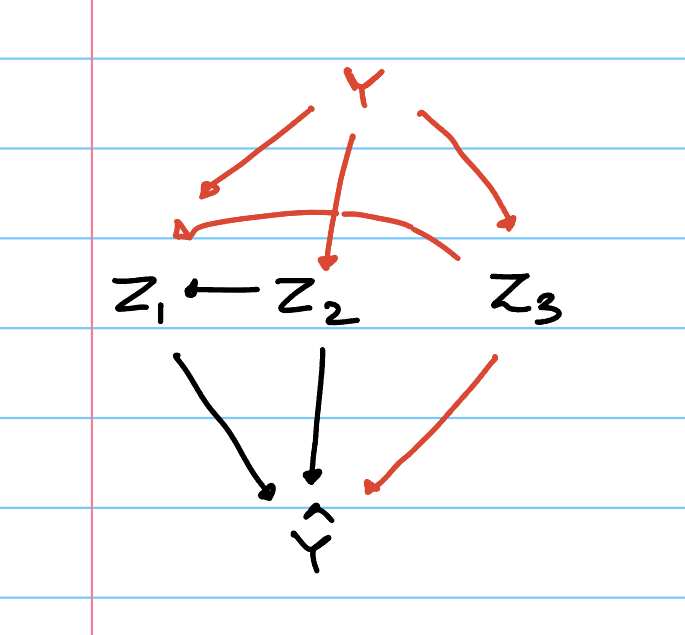
\includegraphics[scale = 0.2]{Do-SHAP_Counterexample.jpeg}
\end{center}

The SCM for this graph is given as 

\begin{align*}
Y &= \epsilon_Y\\
Z_1 &= \nu_0 + \nu_{1}Z_2 + \nu_{2} Z_3 + \nu_{3} Y + \epsilon_{Z_1}\\
\hat{Y} &= \mu_0Z{_1}Z{_3} + \mu_1Z_1 + \mu_2Z_2 
\end{align*}

In our example we will assume $Z_3$ is omitted, and backdoor adjustment is done using $Z_2$. First we calculate SHAP values with a valid adjustment set.
\subsection{SHAP With Valid Adjustment Set}

The SHAP value for $Z_1$ is given as 
\begin{align*}
\phi_{Z_1} &= \frac{0!2!}{3!}\left\{f^\prime_{\{Z_1\}} - f^\prime_{\phi} \right\} + \frac{1!1!}{3!}\left\{f^\prime_{Z_1, Z_2} - f^\prime_{Z_2} \right\} + \frac{1!1!}{3!}\left\{f^\prime_{Z_1, Z_3} - f^\prime_{Z_3} \right\} + \frac{2!0!}{3!}\left\{f^\prime_{\{Z_1, Z_2, Z_3 \}} - f^\prime_{\{Z_2, Z_3 \}}\right\}
\end{align*}

Computing each of the individual pieces
\begin{align*}
f^\prime_{\phi} &= \mathbb{E}[f^\prime(Z_1, Z_2, Z_3)] = \mu_0 \mathbb{E}[Z_1Z_3] + \mu_1\mathbb{E}[Z_1] + \mu_2\mathbb{E}[Z_2]\\
f^\prime_{\{Z_1\}} &= \mathbb{E}[f^\prime(z_1, Z_2, Z_3)] = \mu_0 z_1 \mathbb{E}[Z_3] + \mu_1z_1 + \mu_2\mathbb{E}[Z_2]\\
f^\prime_{\{Z_1, Z_2\}} &= \mathbb{E}[f^\prime(z_1, z_2, Z_3)] = \mu_0 z_1 \mathbb{E}[Z_3] + \mu_1z_1 + \mu_2 z_2\\
f^\prime_{\{Z_2\}} &= \mathbb{E}[f^\prime(Z_1, z_2, Z_3)] = \mu_0 \mathbb{E}[Z_1Z_3] + \mu_1\mathbb{E}[Z_1] + \mu_2 z_2\\
f^\prime_{\{Z_1, Z_3\}} &= \mathbb{E}[f^\prime(z_1, Z_2, z_3)] = \mu_0 z_1 z_3 + \mu_1z_1 + \mu_2 \mathbb{E}[Z_2]\\
f^\prime_{\{Z_3\}} &= \mathbb{E}[f^\prime(Z_1, Z_2, z_3)] = \mu_0 z_3\mathbb{E}[Z_1] + \mu_1\mathbb{E}[Z_1] + \mu_2 \mathbb{E}[Z_2]\\
f^\prime_{\{Z_1, Z_2, Z_3\}} &= \mathbb{E}[f^\prime(z_1, z_2, z_3)] = \mu_0 z_1 z_3 + \mu_1z_1 + \mu_2 z_2\\
f^\prime_{\{Z_2, Z_3\}} &= \mathbb{E}[f^\prime(Z_1, z_2, z_3)] = \mu_0 z_3\mathbb{E}[Z_1] + \mu_1\mathbb{E}[Z_1] + \mu_2 z_2\\
\end{align*}

And this gives us the following SHAP value for $Z_1$
\[
\phi_{Z_1} = \frac{1}{2}\Bigg\{ \mu_0 z_1\mathbb{E}[Z_3] - \mu_0 \mathbb{E}[Z_1 Z_3] + \mu_0 z_1 z_3 - \mu_0z_3 \mathbb{E}[Z_1] \Bigg\}  + \mu_1 \Bigg\{z_1 - \mathbb{E}[Z_1] \Bigg\}
\]

\subsection{SHAP With Invalid Adjustment Set}

In this case, the SHAP value for $Z_1$ is
\[
\phi_{Z_1} = \frac{0!1!}{2!}\Big\{ f^\prime_{\{Z_1\}} - f^\prime_{\phi}\Big\}  + \frac{1!0!}{2!}\Big\{f^\prime_{\{Z_1, Z_2 \}} - f^\prime_{\{Z_2 \}}\Big\}
\] 

Computing these with $Z_3$ missing 
\begin{align*}
f^\prime_{\phi} &= \int f^\prime(Z_1, Z_2, Z_3)p(Z_1, Z_2) = \mu_0 Z_3\mathbb{E}[Z_1] + \mu_1\mathbb{E}[Z_1] + \mu_2\mathbb{E}[Z_2]\\
f^\prime_{\{Z_1\}} &= \int f^\prime(z_1, Z_2, Z_3)p(Z_2) = \mu_0 z_1 Z_3 + \mu_1z_1 + \mu_2\mathbb{E}[Z_2]\\
f^\prime_{\{Z_1, Z_2\}} &= f^\prime(z_1, z_2, Z_3) = \mu_0 z_1 Z_3 + \mu_1z_1 + \mu_2 z_2\\
f^\prime_{\{Z_2\}} &= \int f^\prime(Z_1, z_2, Z_3)p(Z_1) = \mu_0 Z_3 \mathbb{E}[Z_1] + \mu_1\mathbb{E}[Z_1] + \mu_2 z_2\\
\end{align*}

And so the incorrect SHAP value will be
\[
\phi_{Z_1} = (z_1 - \mathbb{E}[Z_1])[\mu_0z_3 + \mu_1] 
\]

Now, if in our explicand, $Z_3$ taken on value $Z_3 = -\frac{\mu_1}{\mu_0}$, then the invalid adjustment set SHAP will equal $0$. The valid adjustment set SHAP will be
\[
\phi_{Z_1} = \frac{1}{2}\Big\{\mu_0z_1\mathbb{E}[Z_3] - \mu_0\mathbb{E}[Z_1Z_3] \Big\} + \frac{1}{2}\mu_1\{z_1 - \mathbb{E}[Z_1] \}
\]

Which can be non-zero.

\subsection{Do-SHAP On A Coalition Of Features}
Given a function $f: \mathcal{X} \rightarrow R$, where $\mathcal{X}$ is the support of the input and the prediction belongs to $\mathbb{R}$, and in the case of classification this can be thought of as the value of the score. Given an explicand $\mathbf{x}$ and a distribution $P(X)$ over the features, we have the classical interpretation of SHAP values. Now, for the same $f$, I instead want SHAP values in terms of $Z_i$'s. This corresponds to setting $v(S) = \mathbb{E}[f(X) \mid do(Z_S = z_S)]$. This would then mean that
\[
v(\mathbf{Z}) = \mathbb{E}[f(X) \mid do(Z = \mathbf{z})] = \sum_{i = 1}^D \phi_{Z_i}
\]

Now, in order to give this approach meaning, a number of assumptions have to be made, starting with assuming that for every explicand $\mathbf{x}$ there is an underlying $\mathbf{z}_{\mathbf{x}}$. Next, we must ask whether we believe the following holds:
\[
\mathbb{E}[f(X) \mid do(Z = \mathbf{z}_{\mathbf{x}})] = f(X)
\]

Whether this holds or not creates a gap between the function to explain $f$, and the function we get SHAP values for, which may or may not cause trouble. Now this is analyzed in two different settings depending on whether $Z$ comes after $X$ or $Z$ comes before $X$, since causal sufficiency and adjustment sets as well as funky mapping functions may be used to make invalid counterpoints. So, analyzing this on a case by case basis, we start by looking at the case when $Z$ comes after $X$.


\subsubsection{$Z$ After $X$}

In this case, the graph would look like

\begin{center}
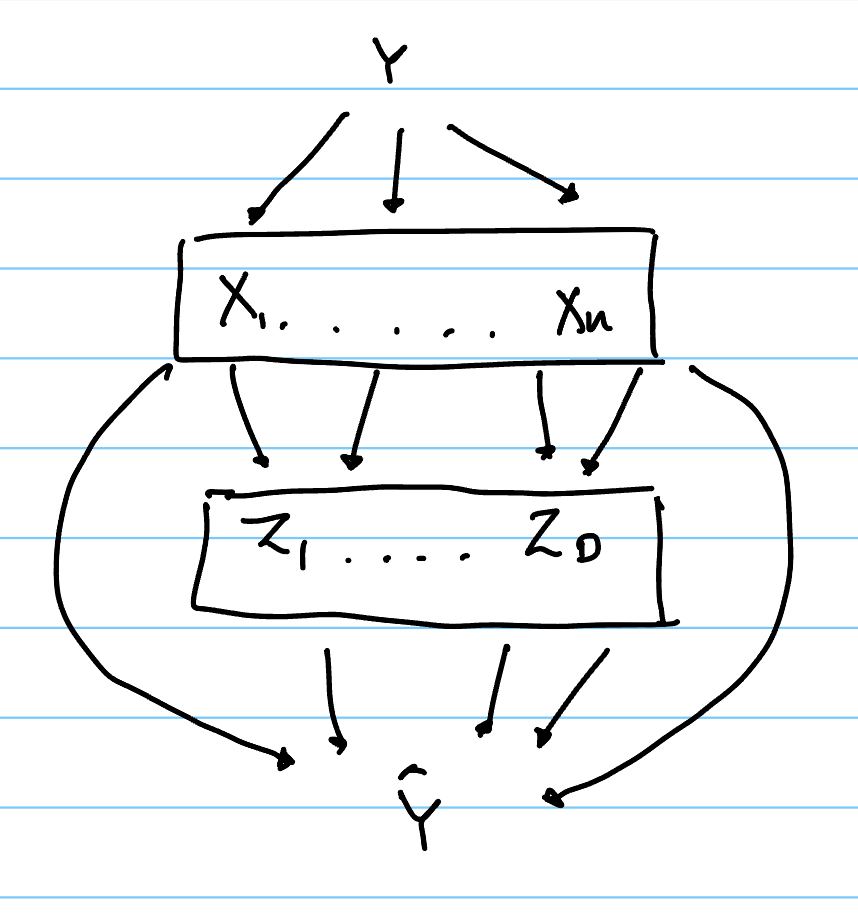
\includegraphics[scale=0.2]{Z_after_X.jpeg}
\end{center}

The first complication arising in this situation is around $\mathbb{E}[f(X) \mid do(Z = \mathbf{z}_{\mathbf{x}})] = f(\mathbf{x})$, since this assumes we are measuring a rich enough feature set that implies no unmeasured confounding, which doesn't hold. Cows on beaches is a prime example of this, where it's not just features of the cow that play a role in the prediction, but rather other image features that aren't in $Z$ will also play a role in the prediction.

First, let's assume causal sufficiency and say the above inequality holds. In this situation, the obstacle to attain correct SHAP value would be estimating the following densities needed to compute $\mathbb{E}[f(X) \mid do(Z_S = z_S) ]$
\begin{align*}
\mathbb{E}_{Z_{\Bar{S}}}[\mathbb{E}[f(X) \mid Z_S = z_S, Z_{\Bar{S}} = z_{\Bar{S}}]]
\end{align*}

Now this could be approximated, but is hard to do and would require some kind of autoencoder nonsense. This still fails in the case where we don't assume causal sufficiency, in which the graph looks like
\begin{center}
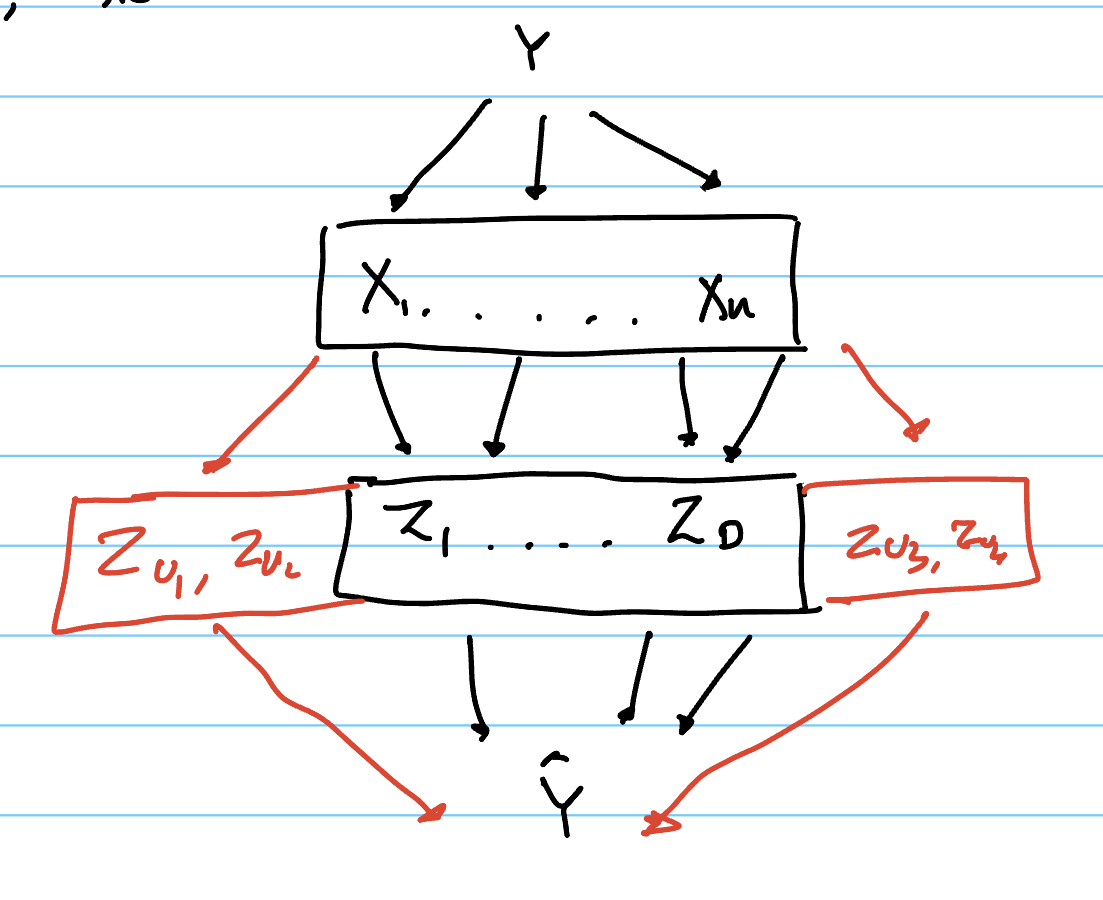
\includegraphics[scale=0.2]{Z_after_X_no_sufficiency.jpeg}
\end{center}

Now one could try fitting models of the $\mathbb{E}[f(X) \mid z_S, X_{\Bar{z}_S}]$, but that is very challenging if not impossible. However, even if we are ultra charitable and say we access a coarse grained prediction function $f^\prime$ in terms of $Z$ that behaves identically to $f(X)$, we have shown previously running SHAP gives errors. 

Now, one could talk about developing a reverse mapping function $h: \mathcal{Z} \rightarrow \mathcal{X}$ and computing $\mathbb{E}[f(X) \mid do(X = h(z_S))]$, however learning such a function is unclear. 

\subsubsection{$Z$ Comes Before $X$}

In this scenario, the causal graph is given as

\begin{center}
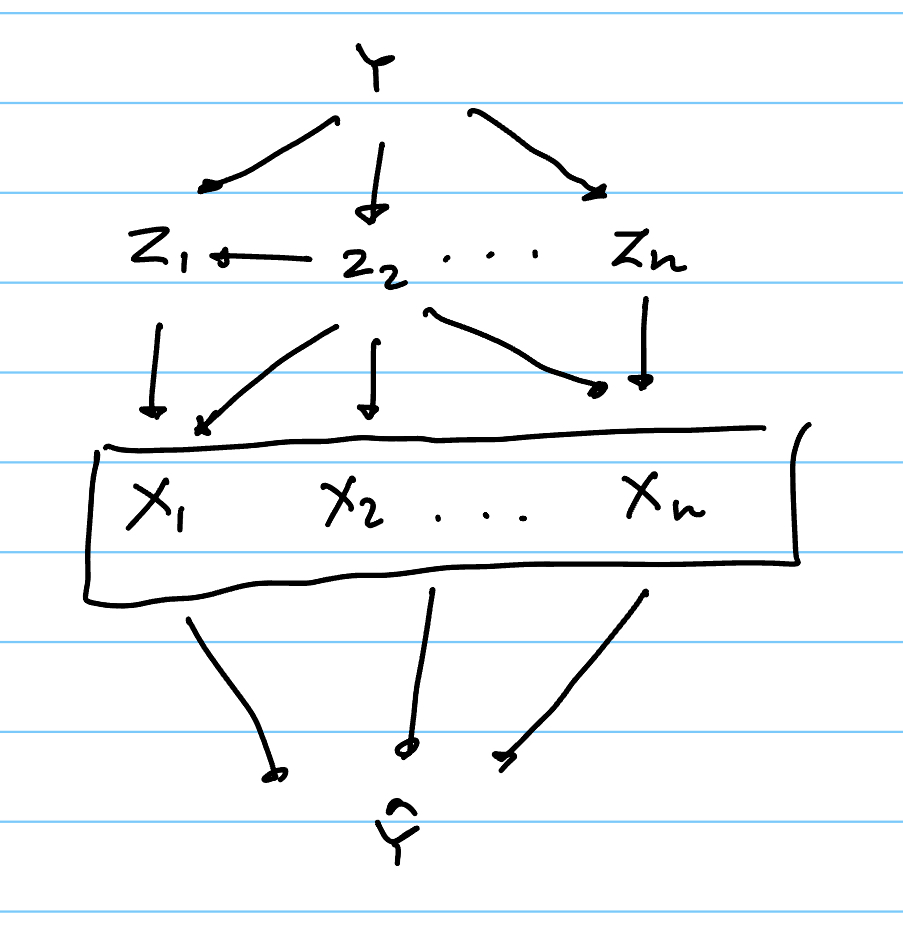
\includegraphics[scale = 0.2]{Z_before_X.jpeg}. 
\end{center}

This setup assumes that for every $\mathbf{x}$  we observe, there is an underlying $\mathbf{z}_\mathbf{x}$. And now we play with the following set of assumptions as these affect the cost function. Namely whether $
\mathbb{E}[f(X) \mid do(Z = z)] = f(X)$ or not, as this describes the link between the function we are providing SHAP values for the function we are actually interested in explaining. 

In this setting, $\mathbb{E}[f(X) \mid do(Z = z)] = f(X)$ is plausible, since given a rich set of $Z$'s we can expect the different variations in $X$ produced mostly disregarded by the classifier. Now the first countere example is obtained by saying, even if we had a coarse grained predictor $f^\prime : \mathcal{Z} \rightarrow \mathbb{R}$, we would still have issues from the counterexample demonstrated before. Now the other other approach involves coputing the interventional expectations directly through a generative model, basically sample $X_i \sim X \mid do(Z_S = z_S)$, and then Monte Carlo integrate over $f(X)$ to obtain the interventional distribution. Now this hinges on being able to learn this high-dimensional distribution, as well as believing the classifier will behave the same even on the synthetic images, which isn't guaranteed given results on adversarial learning etc.
\end{document}
